\documentclass{article}
\renewcommand{\thesection}{\roman{section}} 
\usepackage{amssymb}
\usepackage{graphicx}
\usepackage[nottoc,numbib]{tocbibind}
\usepackage[a4paper, total={6in, 8.75in}]{geometry}
\usepackage{listings}
\usepackage{subcaption}
\usepackage{titling}
\usepackage{pgffor}
\newcommand{\subtitle}[1]{%
  \posttitle{%
    \par\end{center}
    \begin{center}\large#1\end{center}
    \vskip0.5em}%
}
\newcommand{\myparagraph}[1]{\paragraph{#1}\mbox{}\\}

\title{Topics in Privacy \& Security}
\subtitle{Trust-Enhanced Reputation Metrics}
\author{Y1481702}
\date{\today}
\setlength\parindent{0pt}
 
\begin{document}
\begin{titlepage}
\clearpage
\maketitle
\thispagestyle{empty}
\tableofcontents
\end{titlepage}

\lstset{
    tabsize=3,
    numbers=left,
    morekeywords={continue}
}

%Your report should not exceed four A4 pages (minimum font size 11pt), not counting the screenshots and plots from parts (ii) and (iii) of the question, and not counting the references.
%APPROX 1 page per 10 marks!

\section{Description} %5 Marks
%Describe how the tool works
%By means of pseudocode accompanied by a suitable description, explaining how your design takes into account scalability issues (so the tool can handle large input files)
The tool can be run from either the \texttt{run.php} or \texttt{attack.php} scripts in order to calculate reviews or simulate attacks, respectively. For example, from the command-line, \texttt{php run.php} can be called. The program will prompt the user for input of the ratings filename and values of \texttt{MAX\_RATE} and \texttt{ALPHA}.
\\
\textit{N.B. An SQL database must be setup and defined in the \texttt{setup.php} file.}
\\\\
In my implementation of the tool, a number of steps have been taken to help the tool scale.
The tool utilises relational databases to quickly access existing product rating data. The \texttt{CUSTOMERS} and \texttt{PRODUCTS} arrays, as mentioned in the pseudocode, are tables in the database. This means that the tool does not need to store all data in memory, which is usually the most limited resource.
If the tool is needed to scale further, SQL provides \texttt{LIMIT} and \texttt{SKIP} keywords to ensure that memory usage is kept under control.
\\\\
As is visible from the pseudocode of the tool, I have also attempted to cut down on superfluous computation wherever possible.
\begin{lstlisting}
MAX_RATE, ALPHA, FILE = take input from user
CUSTOMERS, PRODUCTS = initialise empty array: []

for each RATING of PRODUCT_J by CUSTOMER_I in FILE:
	if RATING made by a new customer:
		CUSTOMERS.append(New CUSTOMER_I with Default Trust Level of 0.5)

	if RATING made of a new PRODUCT:
		PRODUCTS.append(New PRODUCT_J with RATING)
		continue to next RATING
	else:
		Update the Product Rating for PRODUCT_J

	for each CUSTOMER of PRODUCT_J in CUSTOMERS:
		Update the Trust Level of CUSTOMER

	for each PRODUCT bought by CUSTOMERS of PRODUCT_J:
		Update the Product Rating of PRODUCT

\end{lstlisting}

%todo: FIND REFERENCES FOR significant scalability issues of Trust-Based Reputation Systems?
On Line 6 of the above pseudocode, Equation 3 (from the brief) always returns 0.5 when run with an empty set of products. There is no need to run this calculation each time. Not doing so will save us a small amount of compute time. On Line 10, in the case that this rating is for a new product, the algorithm skips the updating of related customers and products as this will have little effect. This is because, if a product only has one customer, its overall rating is the same as that customer's rating.
\\\\
The loops to update customer trust levels and product ratings on Lines 14 and 17 respectively, are kept to a minimum by filtering down to only updating trust levels of customers that bought the newly rated product. This is important as these nested loops are the part of the program with the worst worst-case complexity. For efficiency, the final implementation need to take care to ensure that each of customer and product is updated only once. If required, further steps to reduce runtime that have not been taken in my implementation, could include only updating Product Ratings (Line 18) if the customer trust levels have changed significantly and running trust level (Line 15) and product rating (Line 18) updates in different, parallel threads.
\\\\
As systems scale, they are more likely to become the target of a form of cyber attack. Prepared statements have been used to sanitise inputs whenever input data from outside the program's control is entered into the database. This should successfully protect against SQL injection attacks.

\section{Analysis} %15 Marks
\label{analysis}
%Use the tool with MAX_RATINGS=5 to analyse the effect of using \alpha=1, \alpha=1.5, \alpha=2 and \alpha=5 on the overall product ratings from the input file Q2Ratings.txt.

%Include screenshots of the tool output;
A tool has been created to provide overall product ratings from an input file. Screenshots of the tool output for the text-file \texttt{Q2Ratings.txt} are shown in Fig. \ref{fig:tool_output}.
%and plots of the overall ratings of the products with IDs 4, 7 and 29 for these \alpha values.
Plots of the ratings for products with IDs 4, 7 and 29 are shown in Fig. \ref{fig:plots_varying_alpha}. For comparison these plots also show the arithmetic mean- the likely rating of the product if a trust-based reputation system is not used.
\\\\
%Discuss the differences between the results obtained for different \alpha values, and between these results and the results obtained for the arithmetic mean.
The products here (Figs. \ref{fig:product4} \& \ref{fig:product29}) show the trust-based reputation system working well.
Product \#4's ratings are all at the bottom end of the scale, with each rating being either 1, 2 or 3. 
Product \#29's ratings are also all similar, but at the top end of the scale, with each rating being 4 or 5.
In these cases the reputation system works well, keeping the overall rating close to the arithmetic mean as the ratings roughly agree how the product should be rated.
\\\\
Product \#7's ratings are much more hit and miss, with every rating being either the minimum rating of 1 or the maximum rating of 5.
Here (Fig. \ref{fig:product7}) we can see the reputation system working to compensate for users' disagreement.
When using the arithmetic mean, each rating is treated with equal weight, so the overall rating falls significantly with each subsequent poor rating.
When using the trust-based system, the first rating it receives (5 from Customer \#16), is treated as the most trustworthy, so it is harder for the subsequent lower ratings to affect overall ratings, when they differ from the overall rating.
The alpha value acts as the tolerance for difference in ratings, lower values of alpha only accept reviews as trusted if they very close to the overall rating.
\\\\
Using a high-value for alpha, $\alpha \geqslant MAX\_RATE$, generally results in a rating that is very similar to the arithmetic mean. The only difference between this trust-based reputation system with $\alpha = 5$ and using the arithmetic mean is that new customers are not fully trusted initially. As customers leave more ratings, their trust level is mindlessly increased whether or not they fit with what is normal within the context of the rest of the population.
While newcomers should always be distrusted\cite{reputation_systems}, it is also important to assess the actions of known customers before upgrading the level of trust they are assigned. As such, it is likely we will want to be slightly more discriminatory against users' actions than this.
\\\\
At the other end of the spectrum, particularly low values of $\alpha$ may not be tolerant enough to account for natural variation of opinion. Clearly some users will be harder to impress than others so allowing reviews to differ by at least some small amount should be expected. If the system is not tolerant enough to variation it becomes too risky for trustworthy users to post new reviews\cite{survey_and_taxonomy} as the system is more likely to significantly lower their trust, especially if their opinions go against the status quo.
\\\\
It's difficult to fully assess how successful the reputation system is at it's aim of predicting the future behaviour of the customers without further data.

\section{Simulated Attacks} %10 Marks
\label{attacks}
%Simulate a self-promoting attack to improve the rating of the product with ID 4 by adding n fake top ratings for this product at the end of Q2Ratings.txt from part (ii) of the question. Each such rating should have a new customer ID, corresponding to a new customer account created by the attacker(s).
Self-promoting attacks of varying sizes have been simulated on product \#4, this is shown by Fig. \ref{fig:graph_promote}.
%Plot the increase in the overall rating achieved by attacks of size n=5, n=10, n=15, n=20 and n=25 for the four \alpha values from part (ii) of the question and for an overall rating based on the arithmetic mean.
%Repeat the experiments for slandering attacks on product with ID 29, plotting the decrease in the overall rating achieved by slandering attacks of size n=5, n=10, n=15, n=20 and n=25 for the four \alpha values from part (ii) of the question and for an overall rating based on the arithmetic mean.
Slander attacks of varying sizes have been simulated on product \#29, this is shown by Fig. \ref{fig:graph_slander}.

\section{Results} %10 marks
%Discuss the results from part (iii) of the question. Explain what value of the parameter \alpha offers the best protection against the attacks you experimented with, and assess the advantages and disadvantages of different values for \alpha.
In Section \ref{analysis}, the advantages and disadvantages of different values of alpha were discussed with regards to normal functioning of the reputation system. Here they will be discussed with regards to the simulated attacks as described in Section \ref{attacks}.
The plots of each attack show that the system is least susceptible to attack when an $\alpha$ value of 2 is used.
This is the case for both self-promotion and slander attacks of \textit{all} sizes in the test-set.
However, it's worth analysing these results in detail before jumping to the conclusion that $\alpha = 2$ is the best value for the system.
%but probably also less susceptible to changes in review
\\\\
Many good reputation systems ensure that newcomers must behave correctly for a given amount of time in order to gain a good reputation. It is important to balance this resilience to attacks with the ease of admittance for new customers.\cite{attack_defense} As discussed in Section \ref{analysis}, values of $\alpha$ that are close to \texttt{MAX\_RATE} do nothing to ensure that users behave correctly. While this will disincentivise the act of creating new accounts for attacks, they allow attackers to perform multiple attacks across a variety of products using the same account in order to increase their trust level. Obviously a compromise is needed.
\\\\
%its hard to distinguish between GENUINE and FAKE reviews
As well as reducing the ease of admittance for new customers, values of alpha that are too low ($\alpha = 1$) don't perform as well as slightly higher values at protecting against attacks. This can be seen clearly in the plots for each attack (Fig. \ref{fig:graph_attacks}).
These lower values tend not to trust several of the genuine reviews as they vary slightly too much from the overall rating.
As such, when attack occurs, the overall rating will begin to deviate from its initial value much more quickly.
%Using values of alpha that ignore new reviews may prevent genuine customer reviewers' opinions from being heard.
\\\\
As this reputation system is fairly primitive, self-promote and slander attacks still have significant effects on the overall rating, with even the most effective value of alpha allowing the attack to change the rating by at least 1. As larger and larger attack sizes are used, the attacker is able to have a significant effect on the product's overall rating. Furthermore, if the attacker has knowledge of the system, they would know that a more effective attack vector could be to submit reviews that are equal to $\alpha$ added to, or subtracted from, from the overall rating as the rating is slowly lowered. A significantly better system is needed to combat these forms of attack. In particular, the ability to find proof of successful transactions, as well as preventing the hacker from obtaining multiple identities, as has been the case in both of these attacks, will be significantly more effective in mitigating both self-promoting and slander attacks.\cite{attack_defense}
\\\\
In conclusion, it seems that $\alpha = 2$ is the most effective value for the system after all. It provides a compromise by ignoring as few genuine reviews as possible while still defending well against different types of attack.
Further work should also be done in order to assess the impact that other forms of attack could have on this reputation system.
For example, as the system uses the current trust level of the reviewer to calculate overall product reviews, it could be particularly susceptible to a whitewashing attack. This is where the reviewer posts malicious or self-promoting reviews and then attempts to repair their reputation afterwards\cite{attack_defense}.

\newpage
\raggedright
\bibliography{Report}{}
\bibliographystyle{ieeetran}
\newpage
\section{Appendix}
%You must attach as an appendix to your single-file submission the source code for the tool. If needed, use a ZIP archive to submit all components of the assessment as a single file.
\begin{figure}[htp]
\centering
\begin{subfigure}{0.49\textwidth}
\centering
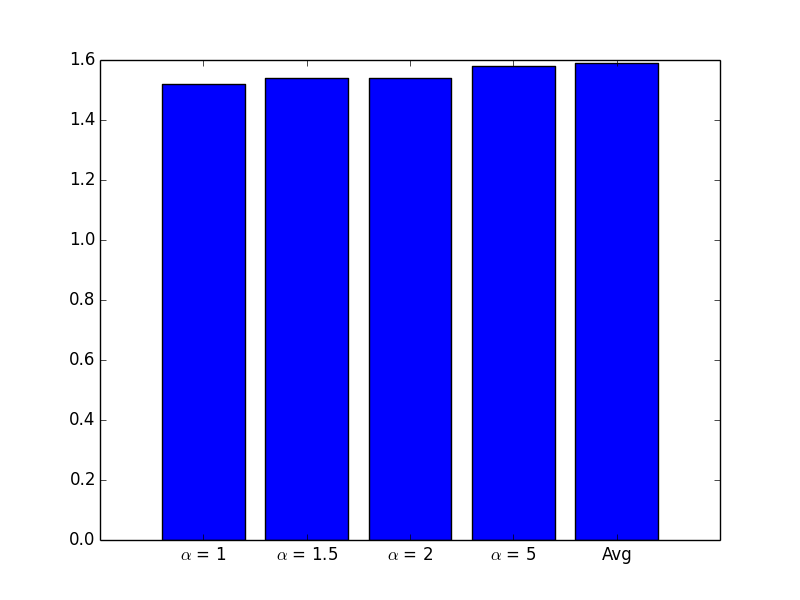
\includegraphics[width=1\textwidth]{Graphs/Product4}
\caption{Product 4}
\label{fig:product4}
\end{subfigure}
\begin{subfigure}{0.49\textwidth}
\centering
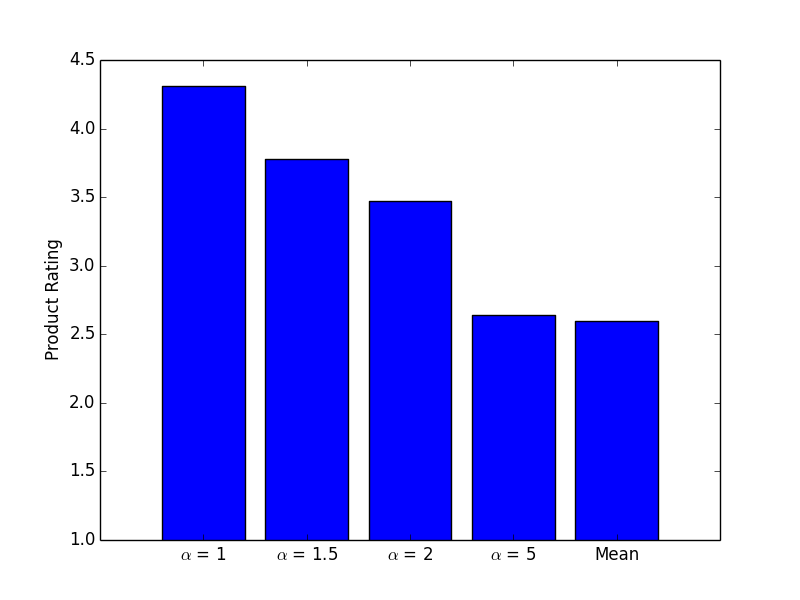
\includegraphics[width=1\textwidth]{Graphs/Product7}
\caption{Product 7}
\label{fig:product7}
\end{subfigure}


\begin{subfigure}{0.5\textwidth}
\centering
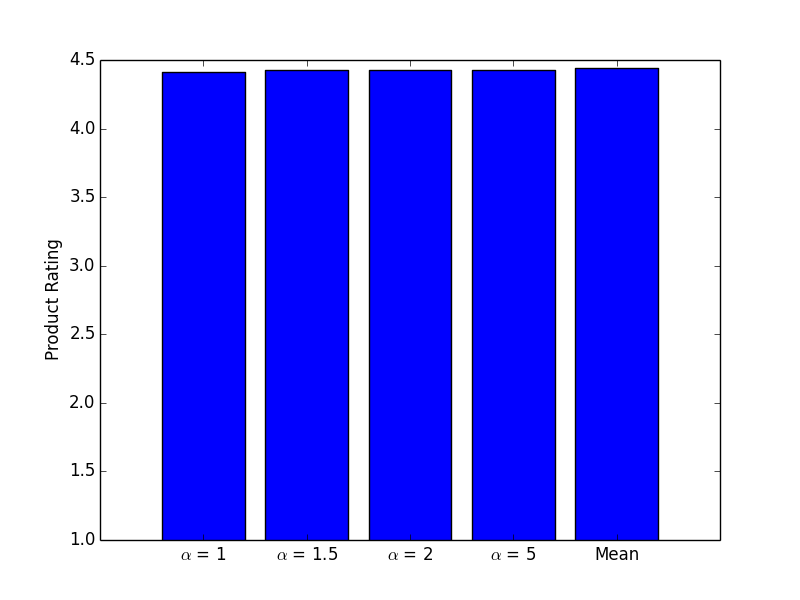
\includegraphics[width=1\textwidth]{Graphs/Product29}
\caption{Product 29}
\label{fig:product29}
\end{subfigure}
\caption{Rating change for varying $\alpha$}
\label{fig:plots_varying_alpha}
\end{figure}


\begin{figure}[htp]
\centering
\begin{subfigure}{0.45\textwidth}
\centering
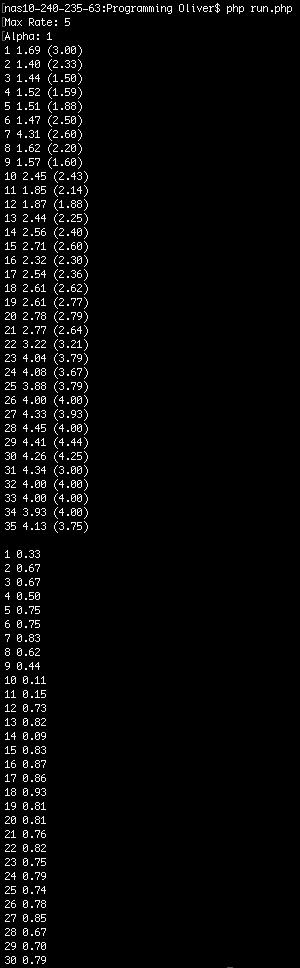
\includegraphics[width=0.9\textwidth]{Screenshots/Alpha1}
\caption{$\alpha = 1$}
\label{fig:screen_alpha1}
\end{subfigure}%
\begin{subfigure}{0.45\textwidth}
\centering
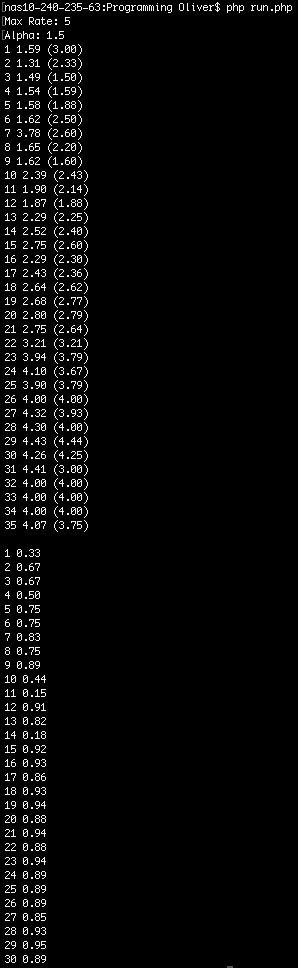
\includegraphics[width=0.9\textwidth]{Screenshots/Alpha1_5}
\caption{$\alpha = 1.5$}
\label{fig:screen_alpha1.5}
\end{subfigure}
\end{figure}

\begin{figure}[htp]\ContinuedFloat
\begin{subfigure}{0.45\textwidth}
\centering
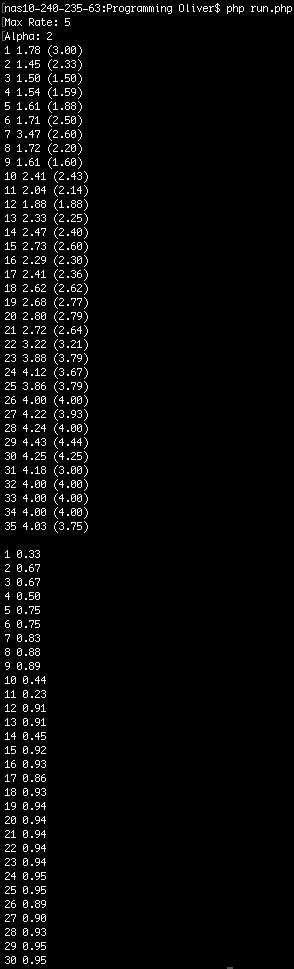
\includegraphics[width=0.9\textwidth]{Screenshots/Alpha2}
\caption{$\alpha = 2$}
\label{fig:screen_alpha2}
\end{subfigure}%
\begin{subfigure}{0.45\textwidth}
\centering
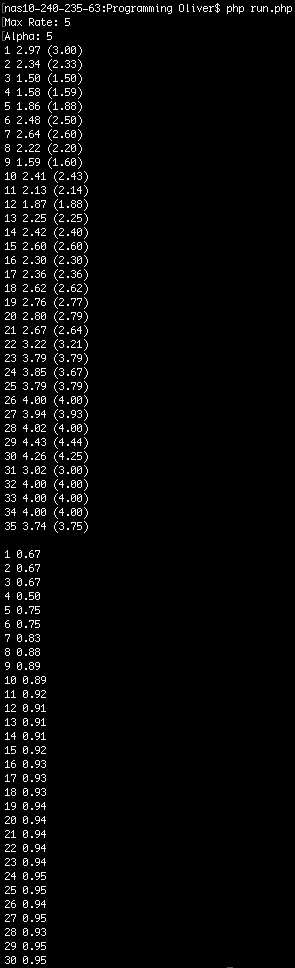
\includegraphics[width=0.9\textwidth]{Screenshots/Alpha5}
\caption{$\alpha = 5$}
\label{fig:screen_alpha5}
\end{subfigure}
\caption{Tool Output for Varying Alpha}
\label{fig:tool_output}
\end{figure}

\begin{figure}[htp]
\centering
\begin{subfigure}{0.85\textwidth}
\centering
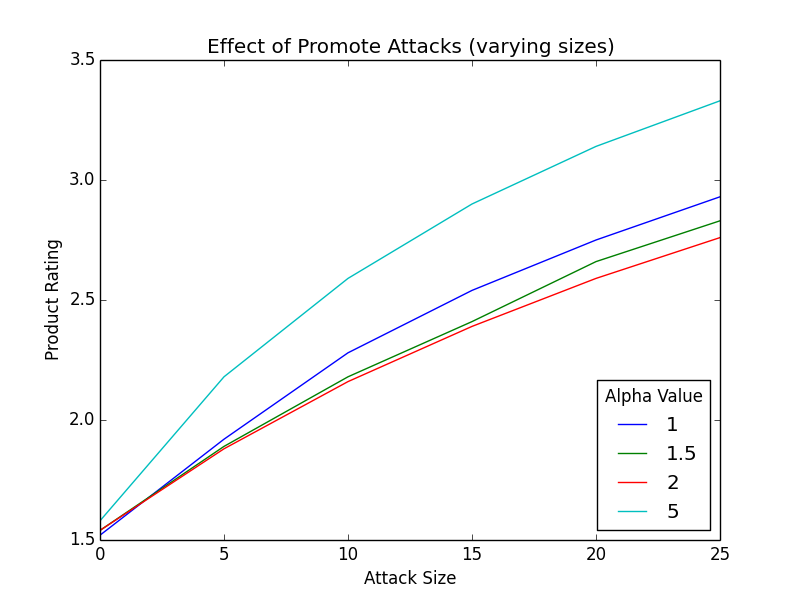
\includegraphics[width=1\textwidth]{Graphs/Promote}
\caption{Effect of Self-Promotion Attacks of Varying Sizes on Product 4}
\label{fig:graph_promote}
\end{subfigure}
\begin{subfigure}{0.85\textwidth}
\centering
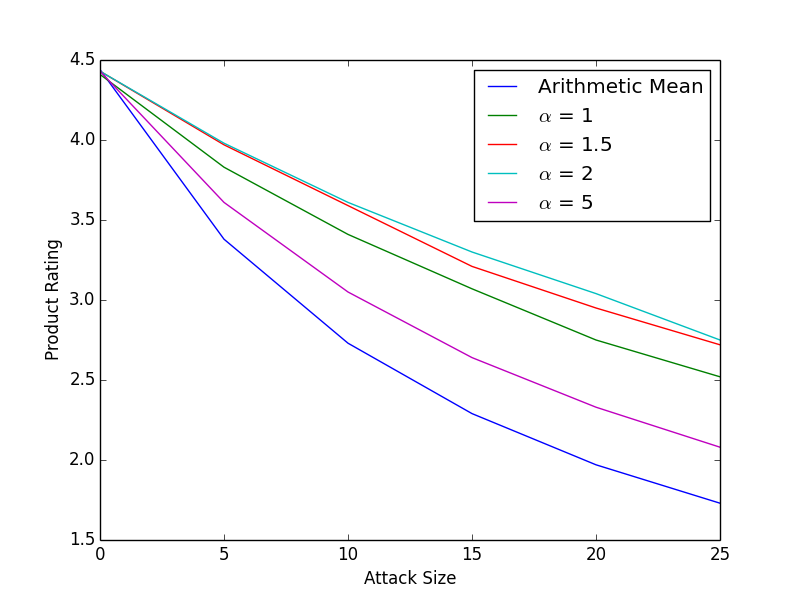
\includegraphics[width=1\textwidth]{Graphs/Slander}
\caption{Effect of Slander Attacks of Varying Sizes on Product 29}
\label{fig:graph_slander}
\end{subfigure}
\caption{Attacks on the Online Store Rating System}
\label{fig:graph_attacks}
\end{figure}

\clearpage
\foreach \x in {run, attack, setup, process, output}
{
	\subsection{\x.php}
	\lstinputlisting[language=PHP]{Programming/\x.php}
}

\end{document}